\label{sec:evsel_paper}

There are various selection criteria applied to the events to remove anomalous signals and noise from the objects for the measurement.
The events must have at least one good primary vertex as described in Sec.~\ref{sec:reconstruction}. 
Furthermore, beam backgrounds
are removed by requiring that events with at least 10 tracks 
have at least 25\% of the tracks satisfying high purity tracking requirements.
Finally, calorimeter noise is removed by timing and pulse shape selections on the signals
from the HB and HE calorimeters. 


For the dijet event selection, events are required to have at least two AK7 jets with
$\pt > 50$ \GeV and $|y| < 2.5$
and each jet must satisfy jet quality criteria \cite{particleflow}.

For the V+jets event selection,
reconstruction of W and Z bosons begins with the identification
and selection of charged leptons and MET described in the previous 
section.  Given the unique signature of a highly boosted vector 
boson recoiling from jets, a minimal selection is sufficient to 
identify highly pure samples of V+jets events. The background is dominated by $\mathrm{t\bar{t}}$ event (and in lower extent from single top events) in the W+jet topology, while in the Z$(\ell\ell)$+jet ($\ell=$ e,$\mu$) analysis the additional constraint on the di-lepton 
mass removes almost completely these backgrounds.  

Candidate \ZtoLL\ decays are reconstructed by combining 
isolated electrons and muons and requiring the dilepton invariant 
mass to satisfy $80<M_{\ell\ell}<100\GeV$.  

Candidate \WtoLN\ decays are identifed primarily by the topology
of a single isolated lepton with high $p_T$ and additional missing energy, with the selection described above.  The
transverse momentum \ptW\ and mass \mtW\ of the W candidate are obtained combining the lepton and the MET transverse four-momomenta components.

The jet mass analysis in V+ jet event is carried on in a boosted kinematic regime, namely $\pt $(V)$> 120$ GeV. We further require the leading jet in the event (independently for each clustering algorithm and jet radius) to have $\pt >$ 125 GeV.
Simply requiring a boosted regime, in addition to the tight isolation cuts on the leptons, is very effective to suppress the QCD background.
In the \WtoLN\ +jet analysis, further QCD rejection is achieved by requiring MET $>$ 50 GeV and $M_T$(W)$>$ 50 GeV.

Figure~\ref{fig:Vjetpt} shows the $p_T$ distribution for Z and W plus jet events for the leading AK7 jet after the selection described above has been applied. 

\begin{figure}[htbp]
\centering
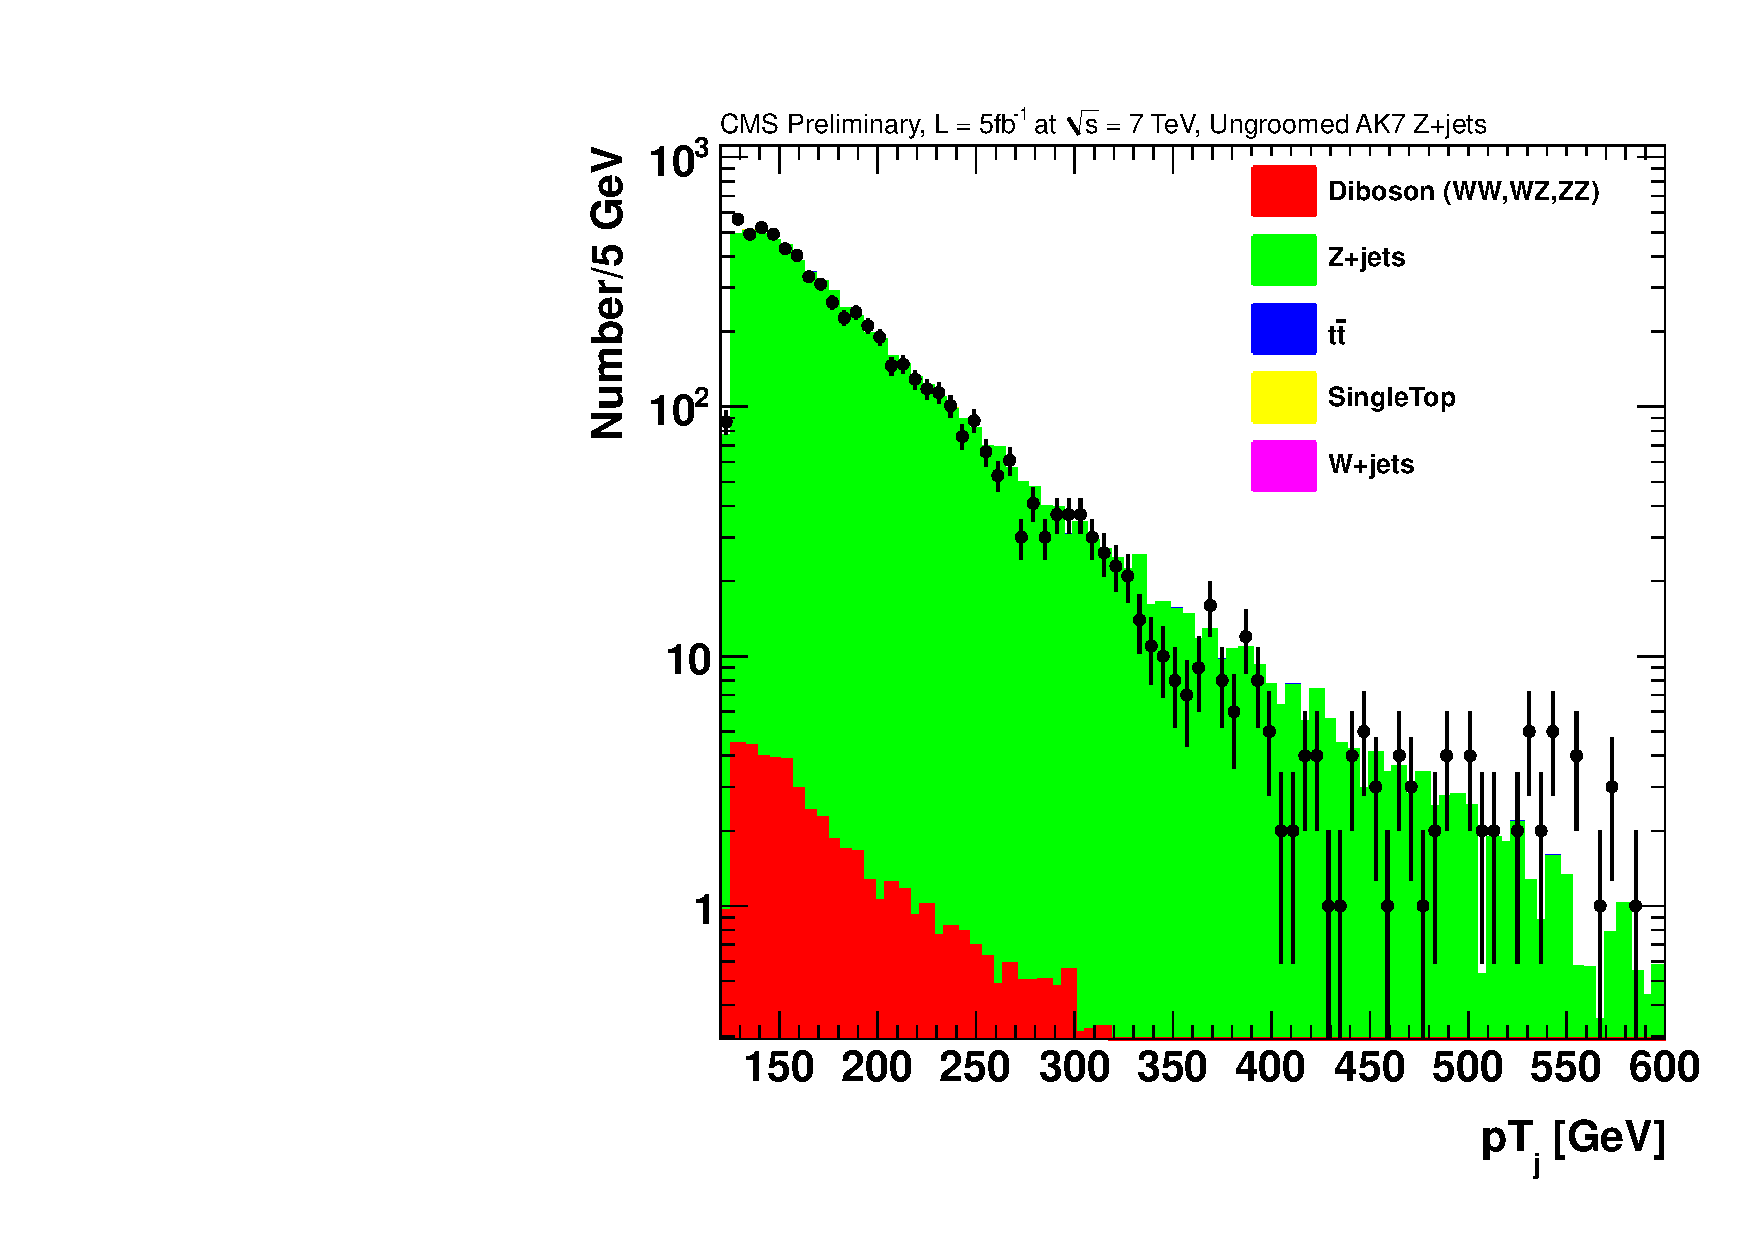
\includegraphics[width=0.495\textwidth]{figs/jetptZ_ak7.pdf}
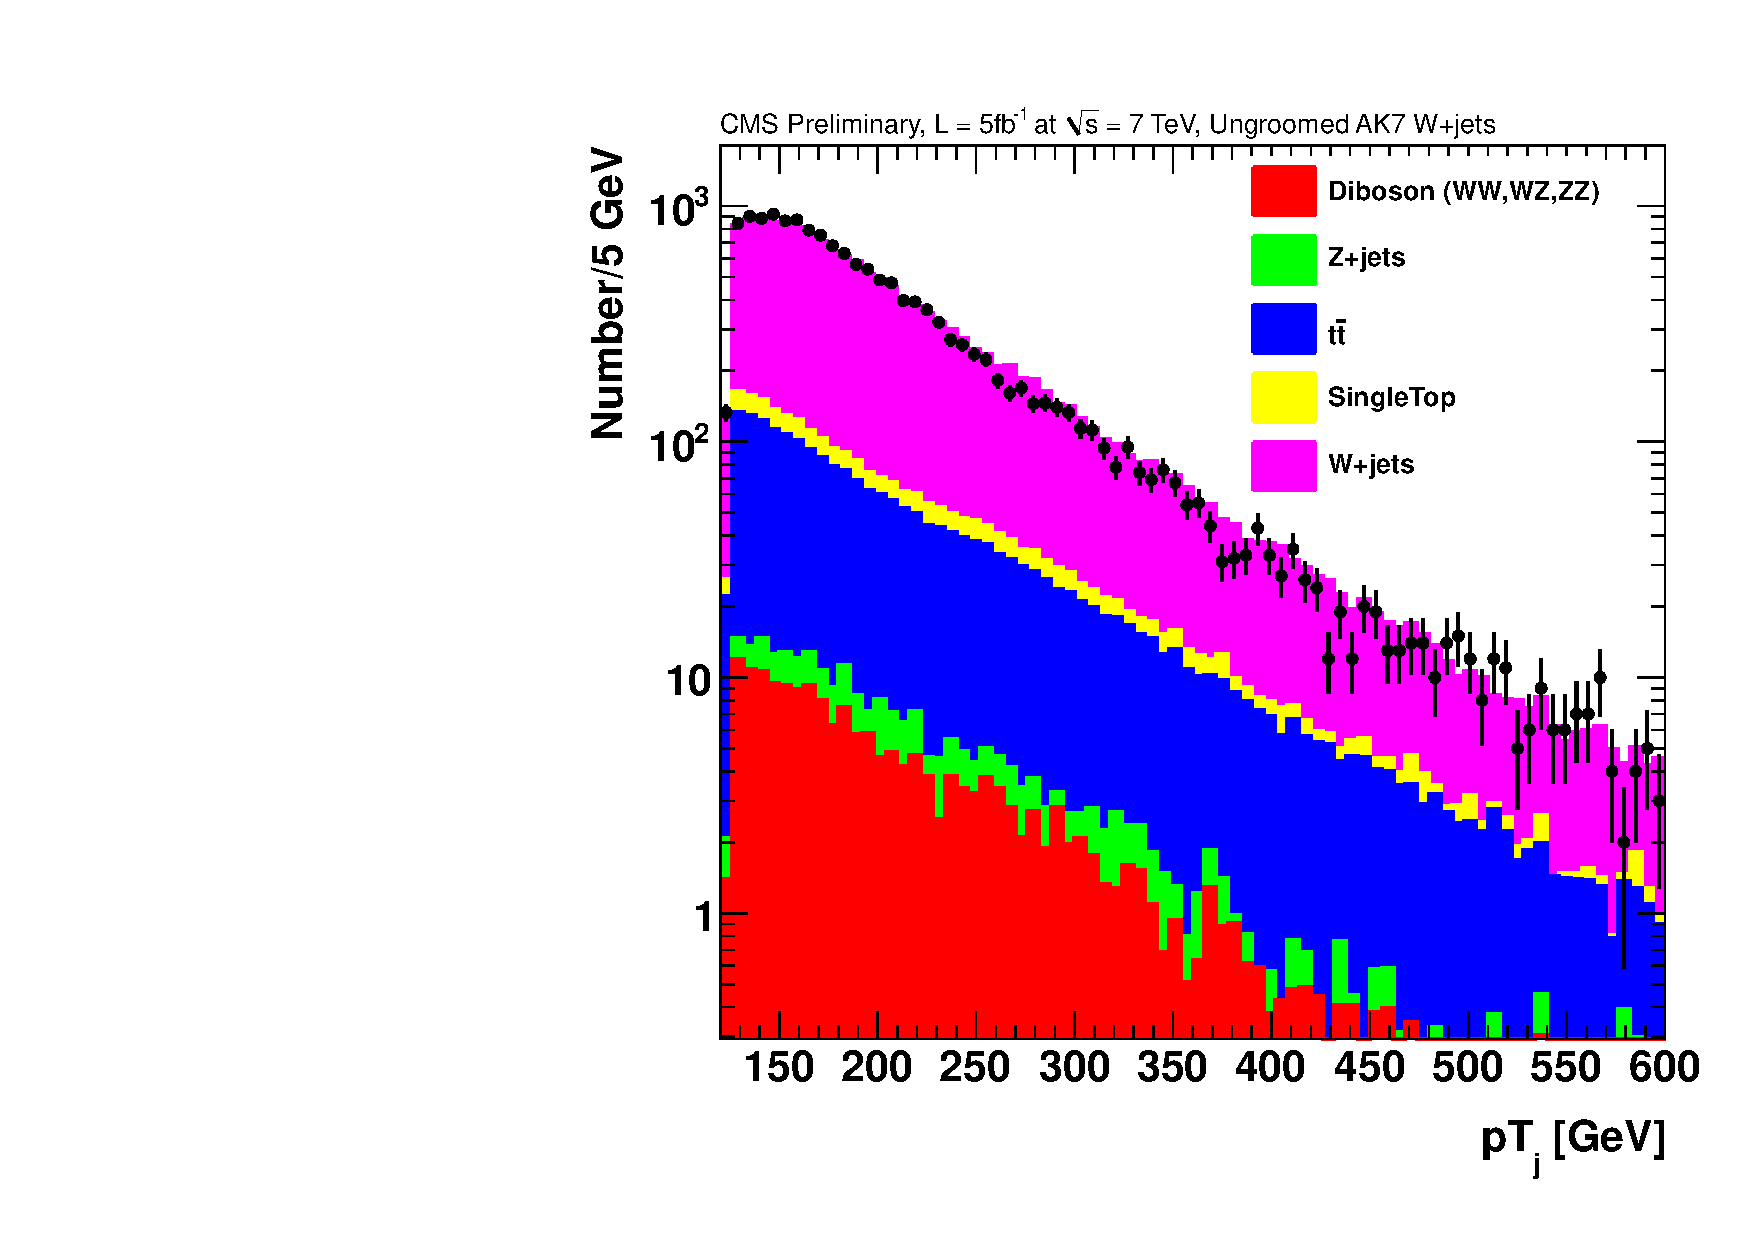
\includegraphics[width=0.495\textwidth]{figs/jetptW_ak7.pdf}
\caption{$p_T$ distribution for the leading AK7 jet in Z and W plus jet event passing the selection criteria.
\label{fig:Vjetpt}}
\end{figure}


After the selection, the Z+jet sample has a purity of about 99\%, with 1\% contamination form di-boson events. The W+jet sample is about 82\% pure, with backgrounds from $\mathrm{t\bar{t}}$ events (13\%), single top (3\%), di-boson and Z plus jets (1\% each). These backgrounds are subtracted based on their MC prediction from the final jet mass distributions before doing the unfolding procedure.
 

